\documentclass[conference]{IEEEtran}
\usepackage{graphicx}
\usepackage{amsmath}
\usepackage{cite}
\graphicspath{{../figures/}{../../outputs/}}

\begin{document}

\title{When Does Classical Image Processing Help a Learned OCR Engine? A Controlled Study on Degraded Insurance Claim Invoices}

\author{\IEEEauthorblockN{Shubham Verma (23CS3052)}
\IEEEauthorblockA{Department of Computer Science and Engineering\\
Rajiv Gandhi Institute of Petroleum Technology\\
Jais, Amethi, India\\
23cs3052@rgipt.ac.in}
\and
\IEEEauthorblockN{Digdarshan Mishra (23CS3024)}
\IEEEauthorblockA{Department of Computer Science and Engineering\\
Rajiv Gandhi Institute of Petroleum Technology\\
Jais, Amethi, India\\
23cs3024@rgipt.ac.in}}

\maketitle

\begin{abstract}
Insurance claim forms and invoices reach an insurer as scans or phone photographs that are skewed, unevenly lit, noisy, blurred or faint. Document-image preprocessing is routinely placed in front of OCR, but most of it was designed for classical engines. We measure which classical digital image processing (DIP) stages actually help a modern learned OCR engine. We generate synthetic A4 invoices with exact ground-truth text, degrade them under seven controlled conditions, and compare five preprocessing pipelines built from grayscale conversion, noise-adaptive denoising, morphological illumination correction, contrast stretching, CLAHE, projection-profile deskewing and adaptive thresholding. Over 20 pages per condition, deskewing reduces the character error rate (CER) from 0.264 to 0.016, and illumination correction rescues a global Otsu threshold (CER 0.458 to 0.015). On already-readable pages the learned engine does as well without preprocessing, while denoising, contrast stretching and especially binarisation (CER 0.313 on clean pages) reduce accuracy. Preprocessing should therefore be applied selectively, according to measured page defects.
\end{abstract}

\begin{IEEEkeywords}
document image processing, OCR, deskewing, illumination correction, binarisation, non-local means
\end{IEEEkeywords}

\section{Introduction and Problem Statement}
Automated claim intake depends on reading claim numbers, policy numbers, dates and amounts from scanned documents. Every common acquisition defect raises the OCR error rate: rotation breaks text-line detection, shading confuses thresholding, and noise and blur corrupt character shapes. The usual remedy is a fixed preprocessing chain in front of OCR. Learned OCR engines, however, are trained on varied images and may not need, or may even be harmed by, that chain.

\textbf{Problem.} Given a degraded document image, which classical DIP stages reduce the error of a learned OCR engine, and which do nothing or hurt? The measurable output is the OCR character and word error rate against known ground truth.

\textbf{Contributions.} (i) A controlled benchmark of synthetic invoices with exact ground truth and seven isolated degradation conditions; (ii) a configurable DIP pipeline with defect-gated stages that act only when a measured defect is present; (iii) a quantified comparison of five pipelines, including a leave-one-stage-out ablation, that reports where preprocessing helps and where it harms.

\section{State of the Art}
\textbf{Binarisation.} Otsu's method selects a global threshold that maximises between-class variance of the grey-level histogram~\cite{otsu1979}. Local methods such as Sauvola's adapt the threshold to the neighbourhood mean and deviation and cope better with uneven background~\cite{sauvola2000}; the DIBCO contests benchmark such methods on degraded documents~\cite{dibco2009}.
\textbf{Denoising and contrast.} Non-local means averages similar patches across the image and preserves edges better than local filters~\cite{buades2005}; CLAHE equalises histograms in tiles with a clip limit to avoid amplifying noise~\cite{zuiderveld1994}. Standard treatments of these operations are given in~\cite{gonzalez2018}.
\textbf{Skew.} Projection-profile methods rotate the page over candidate angles and choose the one whose horizontal profile is most sharply peaked~\cite{postl1986}.
\textbf{OCR engines.} Tesseract is a widely used engine whose classical pipeline expects clean binarised input~\cite{smith2007}. PP-OCR combines a learned text detector and a learned recogniser~\cite{du2020}; the RapidOCR engine used here runs PP-OCR models through ONNX Runtime.
\textbf{Gap.} Preprocessing chains are usually tuned for classical engines, and there is little controlled evidence about which stages still help a learned detector--recogniser engine. This work isolates each defect to answer that question.

\section{Dataset}
Real claim documents are private, so we generate synthetic A4 invoices (1240$\times$1754~px, about 150~dpi). Each page has an insurer title, claim, policy, insured-person, claim-type and date lines, a six-row item table, a total and a footer, rendered with random fonts, names and amounts. The ground-truth text is known exactly. We use 20 documents (seed 2026), each degraded under the seven conditions of Table~\ref{tab:degradations}.

\begin{table}[t]
\caption{Degradation conditions}
\label{tab:degradations}
\centering
\small
\begin{tabular}{|l|p{5.6cm}|}
\hline
\textbf{Condition} & \textbf{Degradation} \\
\hline
clean & none \\
blur & Gaussian, $\sigma = 2.2$~px \\
noise & Gaussian (std 28) + 2\% salt-and-pepper \\
unevenLight & directional ramp down to 35\% brightness \\
lowContrast & grey range compressed to 140--190 \\
skew & rotation of 3--8$^\circ$ \\
combined & blur, contrast, light, noise at 40\% severity + 3--8$^\circ$ skew \\
\hline
\end{tabular}
\end{table}

\section{Methodology}
Fig.~\ref{fig:flowchart} shows the pipeline. Every stage except the OCR engine is a classical DIP operation.

\begin{figure*}[t]
\centering
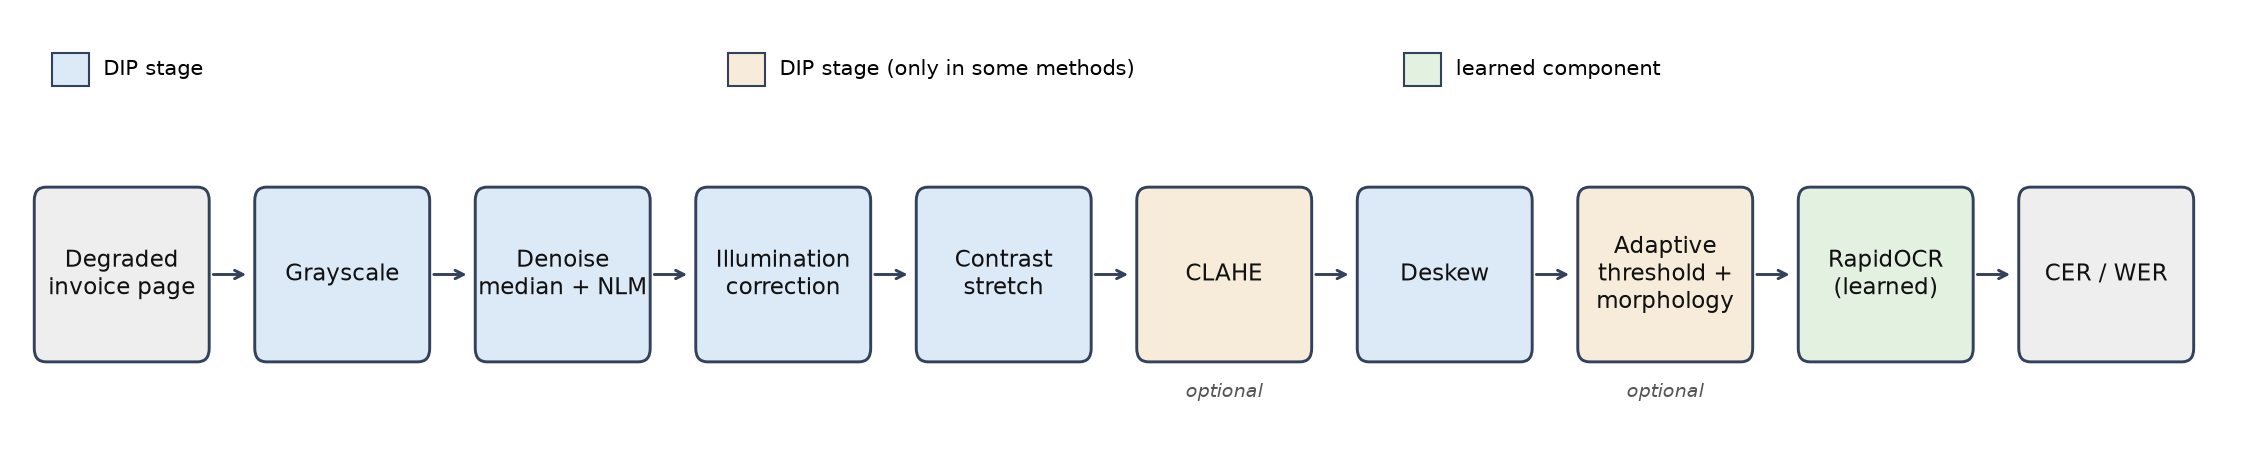
\includegraphics[width=\textwidth]{blockDiagram.png}
\caption{Processing flowchart. Blue: DIP stages; orange: DIP stages used only in some methods; green: learned OCR.}
\label{fig:flowchart}
\end{figure*}

\textbf{Noise-adaptive denoising.} The noise level $\hat\sigma$ is estimated with a wavelet-based robust estimator~\cite{donoho1994}. If $\hat\sigma < 2$ the page is passed through unchanged; otherwise a $3\times3$ median filter removes impulse noise and non-local means~\cite{buades2005} is applied with strength $h = \mathrm{clip}(\hat\sigma, 3, 25)$.

\textbf{Illumination correction.} The background is estimated by a morphological closing with a 41~px elliptical structuring element followed by a 51~px median filter, and the page is divided by it:
\begin{equation}
I_c = 255 \cdot I / B, \quad B = \mathrm{median}_{51}\big(I \bullet S_{41}\big).
\end{equation}

\textbf{Contrast stretch and CLAHE.} Grey levels are mapped linearly so that the median (paper) becomes white and the 0.05th percentile (text) becomes black. CLAHE~\cite{zuiderveld1994} (clip 2.0, 8$\times$8 tiles) is tested as an option.

\textbf{Deskew.} An Otsu text mask $M$ is computed at half resolution; the correction angle is
\begin{equation}
\theta^{*} = \arg\max_{\theta \in [-12^\circ, 12^\circ]} \mathrm{Var}\Big(\sum_{x} R_{\theta}(M)(x, y)\Big),
\end{equation}
searched in 0.5$^\circ$ steps and refined in 0.1$^\circ$ steps. Rotations below 0.3$^\circ$ are skipped because resampling blurs glyph edges.

\textbf{Binarisation (optional).} Gaussian adaptive thresholding (block 35, offset 15) followed by a 2$\times$2 opening and closing.

\textbf{Methods compared.} \emph{gray} (baseline); \emph{otsu} (global threshold); \emph{enhanced} (denoise, illumination, stretch, deskew); \emph{enhancedClahe}; \emph{enhancedBinary} (enhanced + adaptive threshold + morphology). Algorithm~1 summarises the enhanced pipeline.

\begin{figure}[t]
\small
\hrule\vspace{2pt}
\textbf{Algorithm 1:} Defect-gated enhancement and evaluation
\vspace{2pt}\hrule\vspace{3pt}
\begin{tabbing}
xx\=xx\=xx\=\kill
\textbf{Input:} page image $I$, ground truth $T$\\
\textbf{Output:} CER, WER\\
1: $I \leftarrow \mathrm{gray}(I)$\\
2: $\hat\sigma \leftarrow \mathrm{estimateNoise}(I)$\\
3: \textbf{if} $\hat\sigma \ge 2$ \textbf{then}\\
4: \> $I \leftarrow \mathrm{NLM}(\mathrm{median}_3(I),\ \mathrm{clip}(\hat\sigma,3,25))$\\
5: $B \leftarrow \mathrm{median}_{51}(\mathrm{close}(I, S_{41}))$;\ $I \leftarrow 255\, I / B$\\
6: $I \leftarrow \mathrm{stretch}(I,\ p_{0.05} \to 0,\ \mathrm{median} \to 255)$\\
7: $\theta^{*} \leftarrow \mathrm{projectionSearch}(\mathrm{otsuMask}(I))$\\
8: \textbf{if} $|\theta^{*}| \ge 0.3^\circ$ \textbf{then} $I \leftarrow \mathrm{rotate}(I, \theta^{*})$\\
9: $\hat T \leftarrow \mathrm{OCR}(I)$ grouped into lines by position\\
10: \textbf{return} $\mathrm{CER}(T, \hat T)$, $\mathrm{WER}(T, \hat T)$
\end{tabbing}
\vspace{-6pt}\hrule
\end{figure}

\textbf{Evaluation.} CER and WER are normalised Levenshtein distances~\cite{levenshtein1966} at character and word level. CER ignores whitespace so that the engine's spacing choices are not counted as errors. We also report PSNR and SSIM~\cite{wang2004} where the image size is unchanged, and the skew-estimation error.

\section{Novelty and USP Using DIP}
(i) \textbf{Defect-gated preprocessing:} each stage first measures the defect it targets (noise level, skew angle) and leaves the page untouched when the defect is absent, which keeps clean pages at the baseline error. (ii) \textbf{Defect-isolated benchmark:} because every degradation is applied in isolation with exact ground truth, accuracy changes can be attributed to a specific DIP stage. (iii) \textbf{Evidence against blanket preprocessing:} the study quantifies where classical stages that suit classical OCR harm a learned engine.

\section{Implementation}
The system is written in Python with OpenCV, scikit-image and RapidOCR. Configuration, degradations, enhancement stages, OCR adapter, metrics and reporting are separate modules; the experiment command regenerates all tables and figures (about 25 minutes on a CPU for 20 documents). Source code: https://github.com/Galaxus21/dipDocOcr.

\section{Results}
Table~\ref{tab:cer} gives the mean CER over 20 documents per condition; Fig.~\ref{fig:cer} plots it and Fig.~\ref{fig:stages} shows the intermediate images.

\begin{table}[t]
\caption{Mean CER (lower is better), 20 pages per condition}
\label{tab:cer}
\centering
\small
\setlength{\tabcolsep}{3.5pt}
\begin{tabular}{|l|c|c|c|c|c|}
\hline
\textbf{Condition} & \textbf{gray} & \textbf{otsu} & \textbf{enh.} & \textbf{+CLAHE} & \textbf{+binary} \\
\hline
clean & 0.015 & 0.034 & 0.015 & 0.015 & 0.313 \\
blur & 0.024 & 0.657 & 0.019 & 0.017 & 0.258 \\
noise & 0.030 & 0.137 & 0.047 & 0.093 & 0.339 \\
unevenLight & 0.017 & 0.458 & 0.015 & 0.015 & 0.312 \\
lowContrast & 0.017 & 0.030 & 0.071 & 0.068 & 0.274 \\
skew & 0.264 & 0.266 & 0.016 & 0.016 & 0.039 \\
combined & 1.000 & 0.992 & 0.937 & 0.944 & 0.983 \\
\hline
\end{tabular}
\end{table}

\begin{figure}[t]
\centering
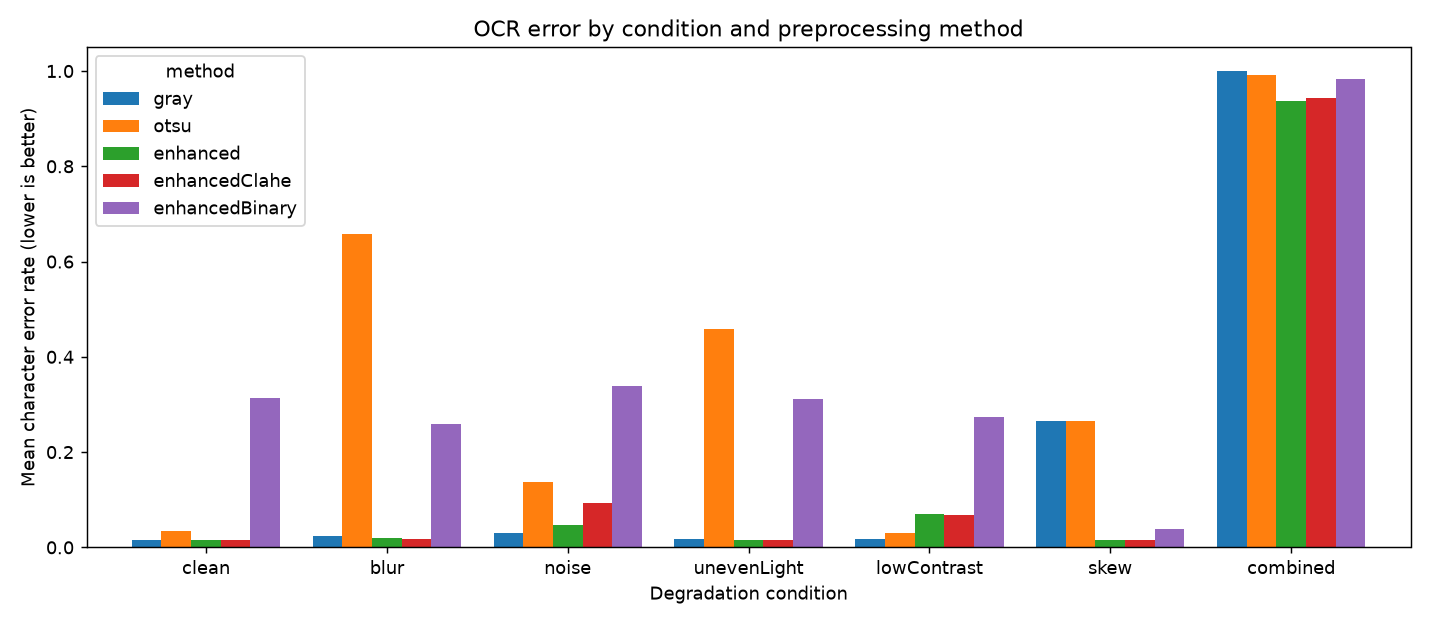
\includegraphics[width=\columnwidth]{cerByCondition.png}
\caption{Mean CER by condition and method.}
\label{fig:cer}
\end{figure}

\begin{figure}[t]
\centering
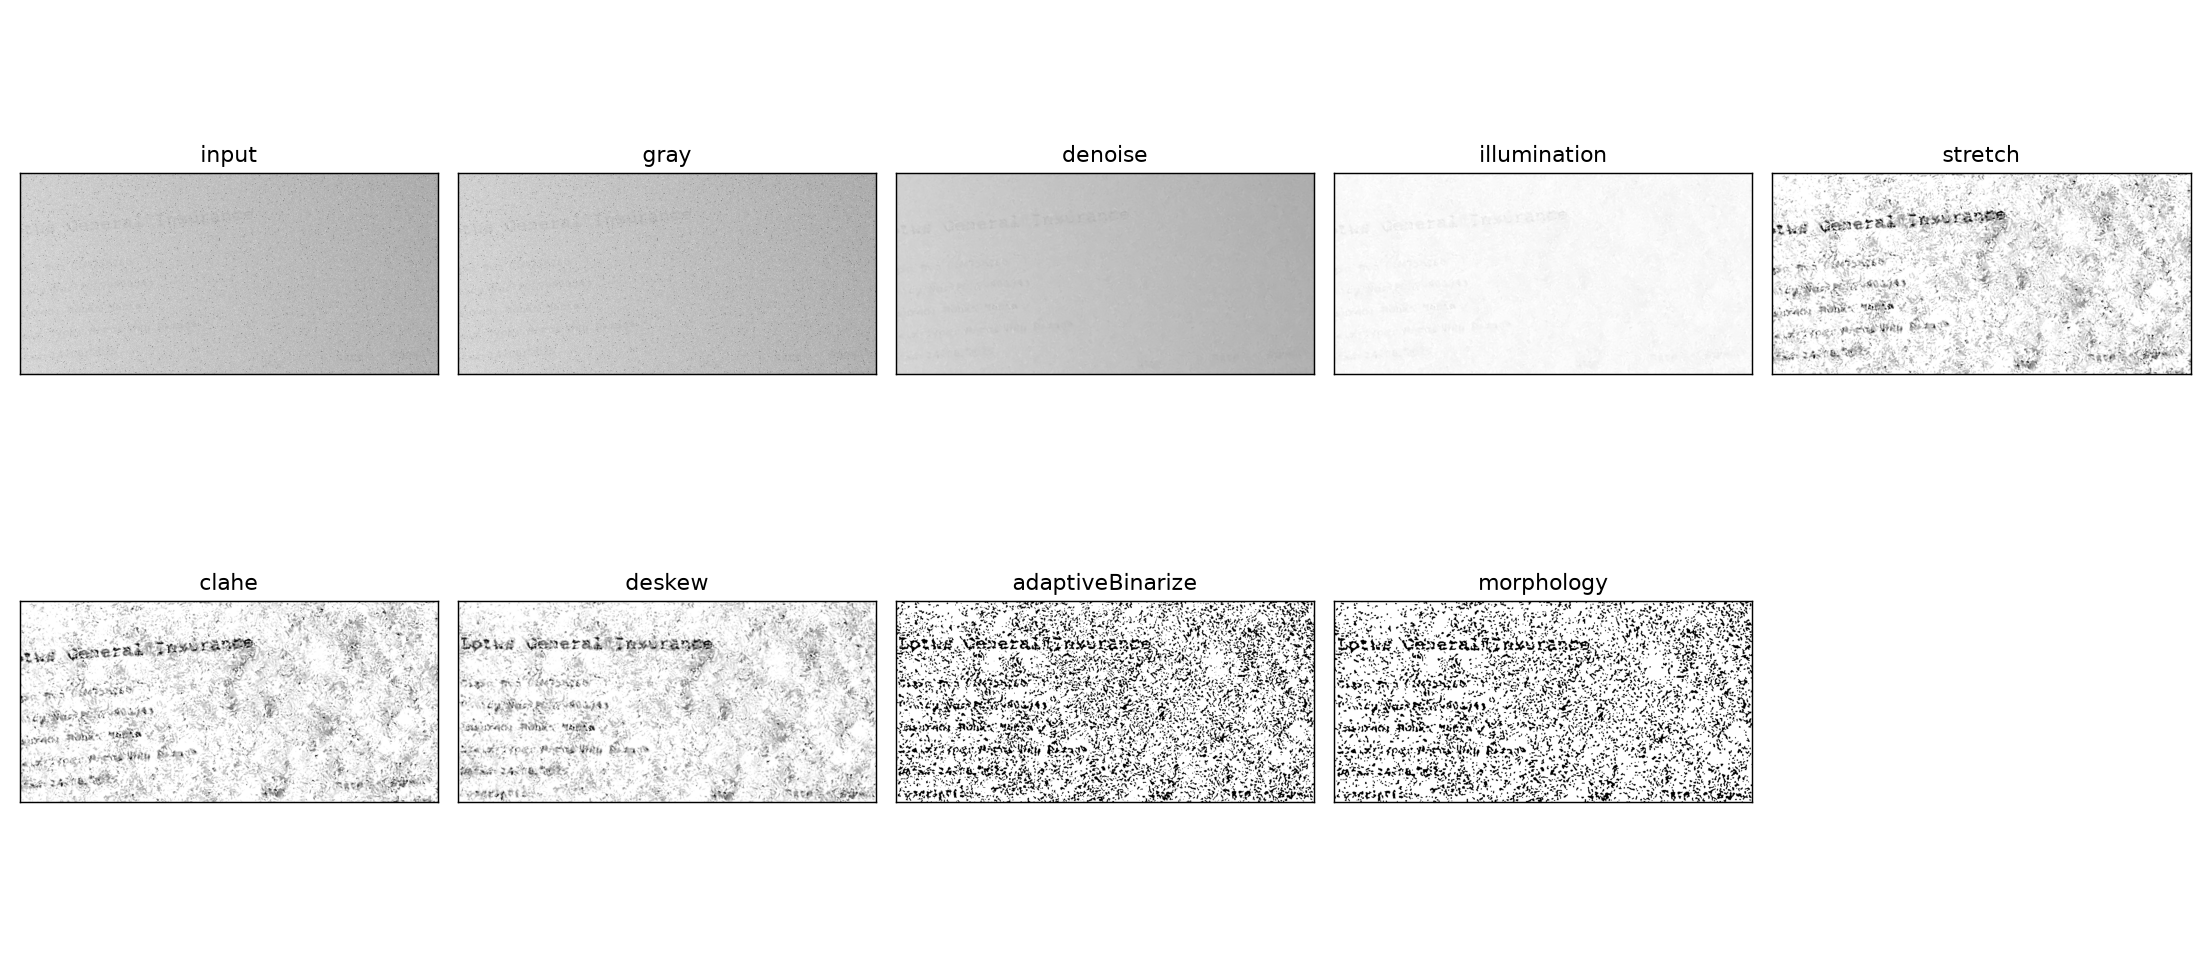
\includegraphics[width=\columnwidth]{pipelineStages.png}
\caption{Intermediate images for one combined-condition page (header region).}
\label{fig:stages}
\end{figure}

\textbf{Where DIP helps.} Deskewing reduces CER on skewed pages from 0.264 to 0.016; the mean skew-estimation error is 0.028$^\circ$ on skewed pages and 0.081$^\circ$ on combined pages. A global Otsu threshold fails under uneven light and blur (0.458 and 0.657), and the enhanced pipeline restores 0.015 and 0.019.

\textbf{Where it does not.} Against the untouched grayscale image, enhancement gives no gain on clean, blurred and unevenly lit pages (0.015--0.024): the learned engine already copes. Enhancement worsens noise (0.030 to 0.047) and low contrast (0.017 to 0.071), as denoising and stretching distort faint strokes. Binarisation discards grey-level cues the recogniser uses (0.313 on clean pages). The combined condition defeats every method (0.94--1.00).

\textbf{Word error rate.} Table~\ref{tab:wer} gives the mean WER. It follows the same pattern but is more sensitive, because a single wrong character in a claim number or amount makes the whole word wrong; on skewed pages deskewing lowers WER from 0.357 to 0.092.

\begin{table}[t]
\caption{Mean WER (lower is better), 20 pages per condition}
\label{tab:wer}
\centering
\small
\setlength{\tabcolsep}{3.5pt}
\begin{tabular}{|l|c|c|c|c|c|}
\hline
\textbf{Condition} & \textbf{gray} & \textbf{otsu} & \textbf{enh.} & \textbf{+CLAHE} & \textbf{+binary} \\
\hline
clean & 0.086 & 0.115 & 0.086 & 0.086 & 0.583 \\
blur & 0.322 & 0.936 & 0.350 & 0.359 & 0.781 \\
noise & 0.204 & 0.579 & 0.364 & 0.604 & 0.641 \\
unevenLight & 0.089 & 0.532 & 0.086 & 0.087 & 0.581 \\
lowContrast & 0.092 & 0.116 & 0.269 & 0.263 & 0.671 \\
skew & 0.357 & 0.377 & 0.092 & 0.095 & 0.202 \\
combined & 1.000 & 0.999 & 0.992 & 0.996 & 1.000 \\
\hline
\end{tabular}
\end{table}

\textbf{Image fidelity.} For the enhanced output, PSNR/SSIM against the clean page are 22.1~dB/0.952 (blur), 26.3~dB/0.666 (noise), 59.1~dB/1.000 (uneven light) and 28.8~dB/0.987 (low contrast). The low SSIM on noisy pages agrees with the CER increase: the denoised page differs structurally from the clean one even though it looks smoother.

\begin{figure}[t]
\centering
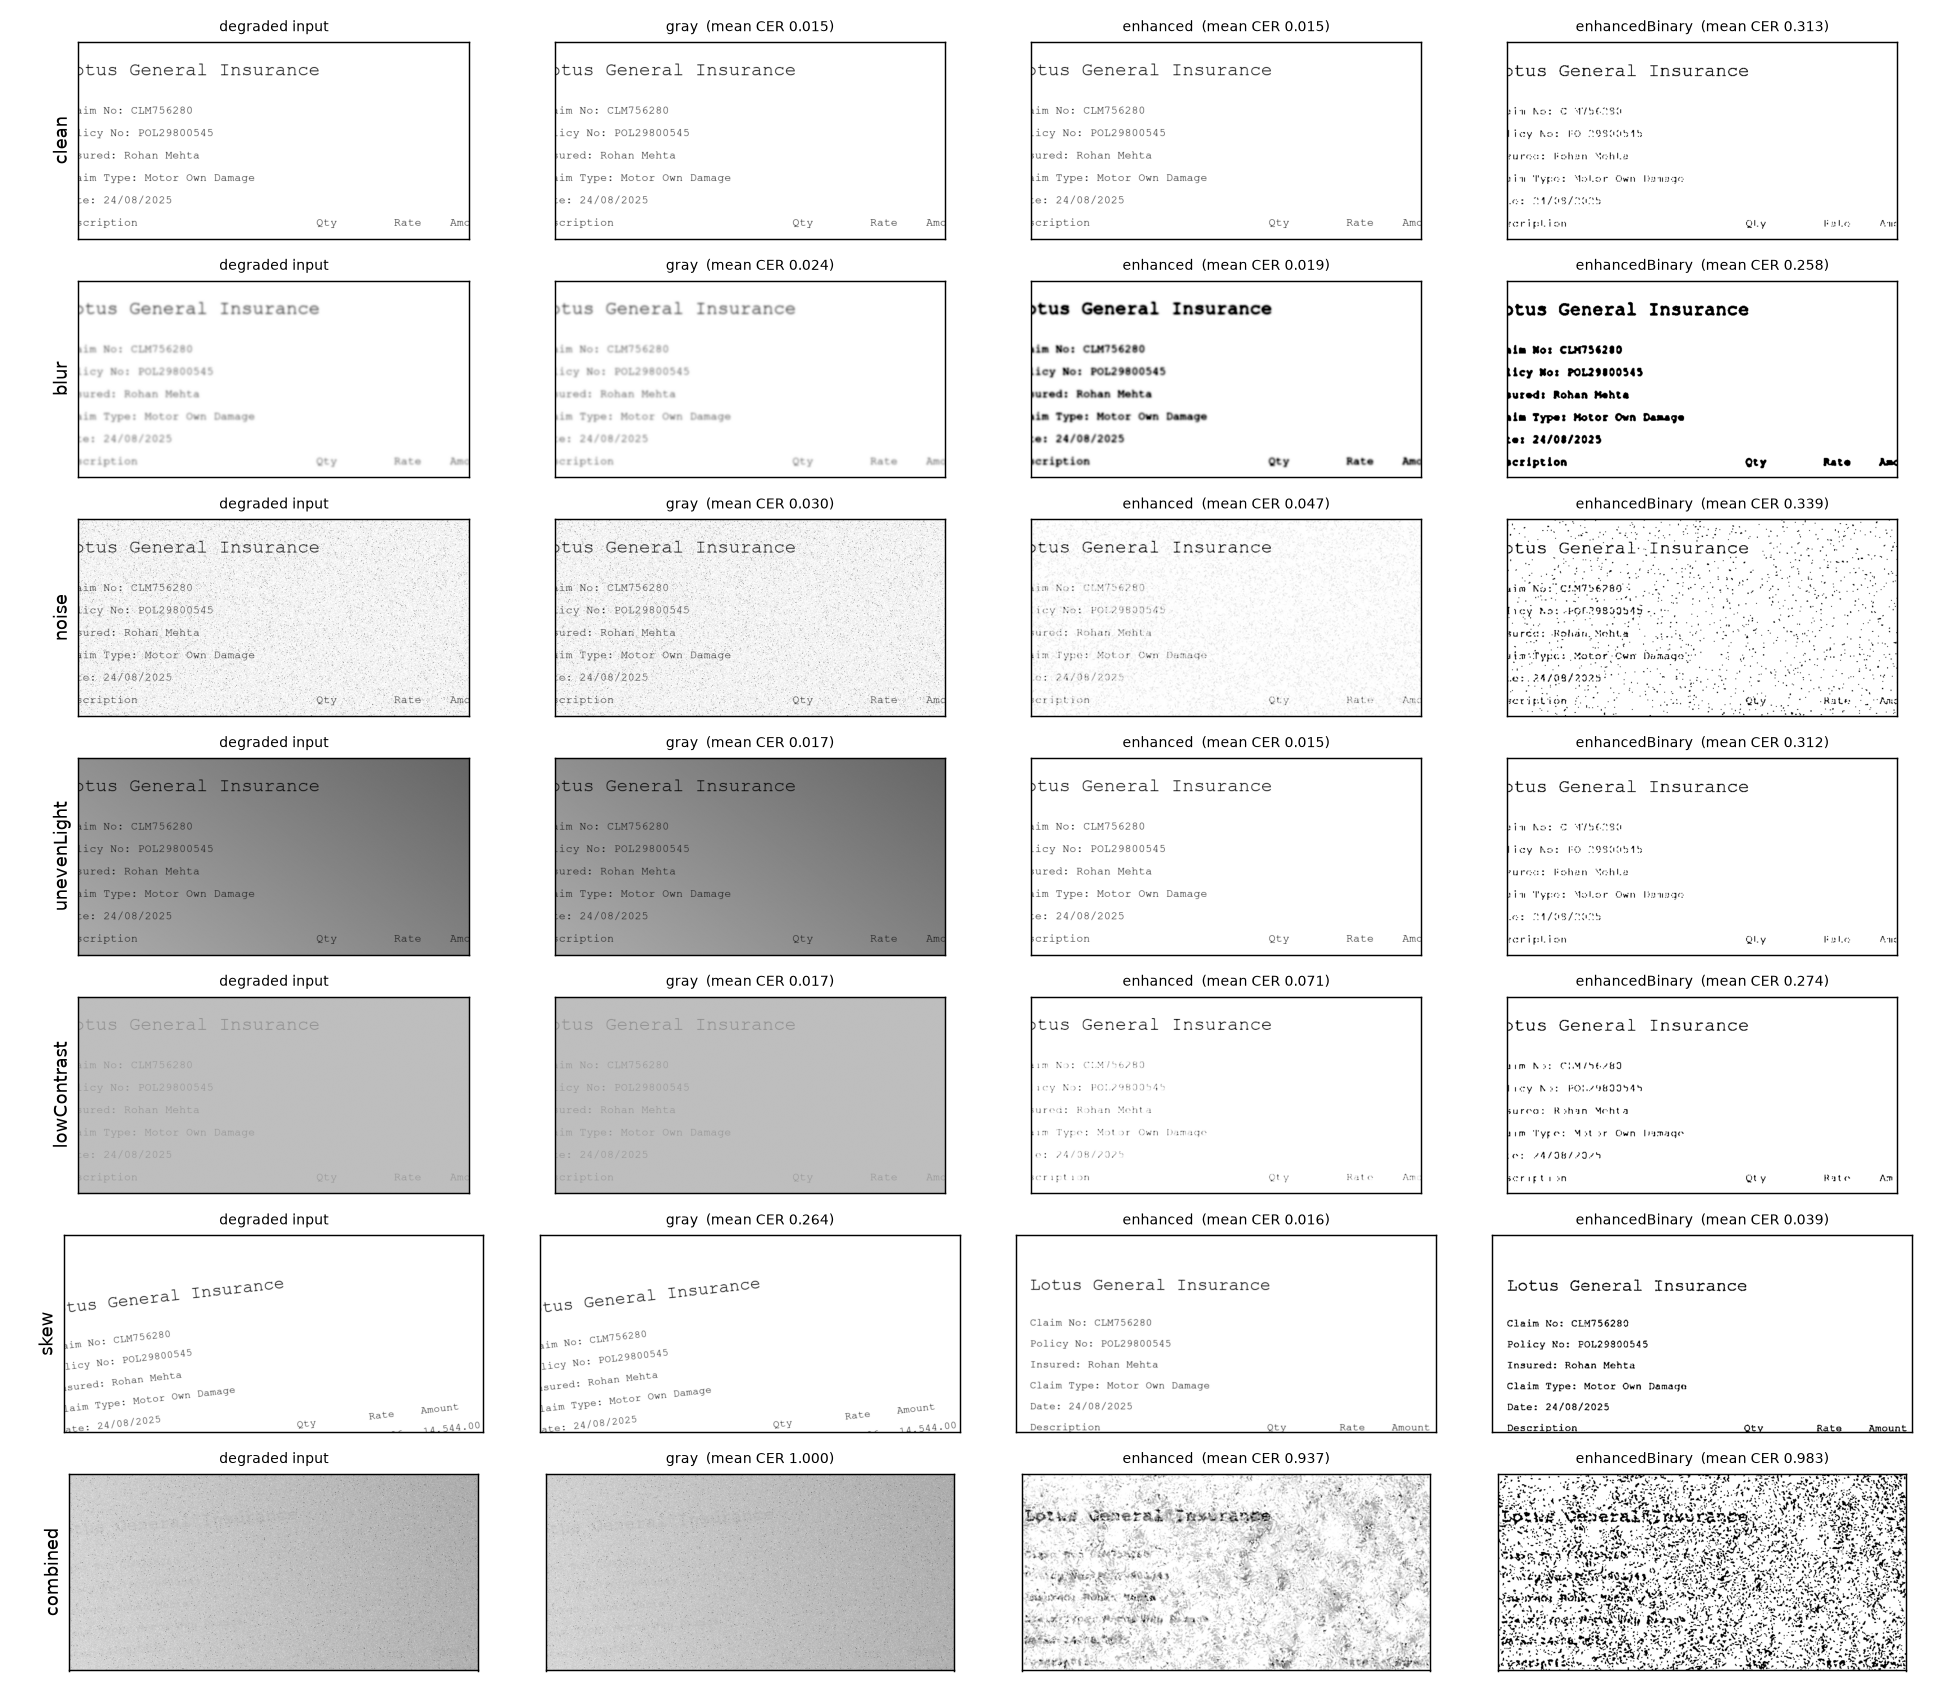
\includegraphics[width=\columnwidth]{beforeAfter.png}
\caption{Degraded input and outputs of gray, enhanced and enhancedBinary for each condition (rows), with mean CER.}
\label{fig:beforeafter}
\end{figure}

\textbf{Ablation.} Fig.~\ref{fig:ablation} shows the leave-one-stage-out ablation on the combined condition. It is uninformative: all variants lie at CER 0.98--0.99 except removing adaptive thresholding (0.909). This is a floor effect, because the combined page is nearly unreadable, not evidence that the other stages are unnecessary.

\begin{figure}[t]
\centering
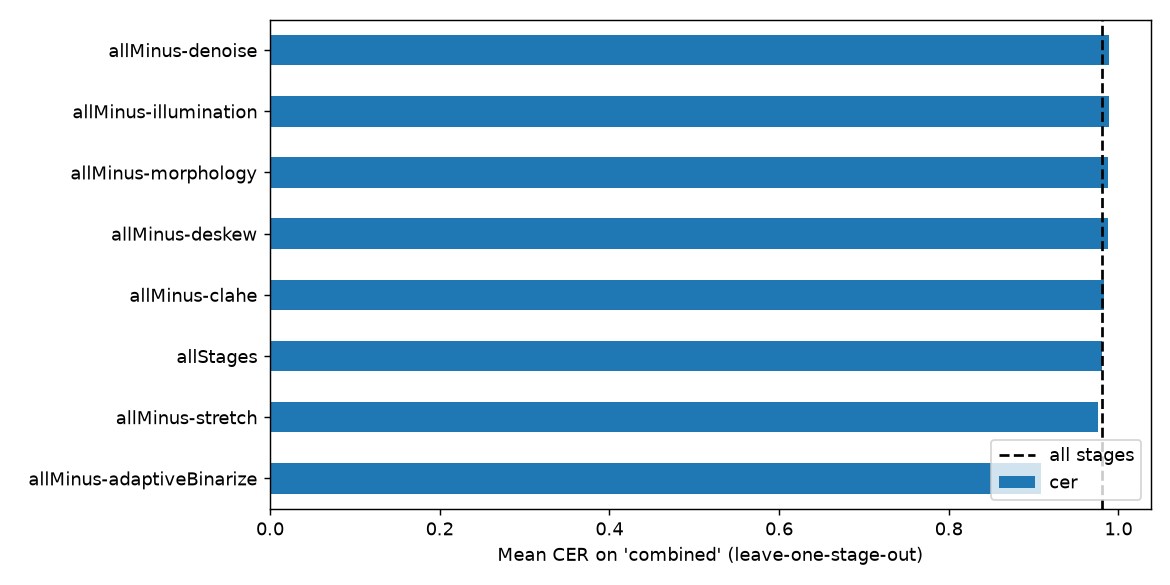
\includegraphics[width=0.92\columnwidth]{ablation.png}
\caption{Leave-one-stage-out ablation on the combined condition.}
\label{fig:ablation}
\end{figure}

\subsection{Failure-case analysis}
Fig.~\ref{fig:beforeafter} shows representative outputs. \emph{Combined pages:} after 40\% blur, contrast loss and shading, the strokes are only a few grey levels darker than the noisy background; the OCR detector finds no text regions on the worst pages and returns an empty string (CER 1.0), so no downstream stage can recover them. \emph{Binarisation:} adaptive thresholding turns residual background texture into black specks and removes the anti-aliased grey edges of strokes (Fig.~\ref{fig:beforeafter}, last column); we attribute the error increase to the recogniser having been trained on grey images. \emph{Low contrast:} we hypothesise that the 0.05th-percentile anchor of the stretch can fall on noise rather than text on a faint page, so the stretch amplifies noise along with text. \emph{Noise:} a likely cause is that non-local means also smooths thin strokes; the raw noisy page is read better. These explanations are not yet tested in isolation.

\section{Limitations}
The pages are synthetic with one layout, so results may not transfer to real scans. Only one OCR engine was tested; a classical engine such as Tesseract would likely respond differently to binarisation. Parameters were adjusted after inspecting pilot pages of the same generator, without a held-out set. With 20 pages per condition, CER differences of a few thousandths are not significant.

\section{Conclusion}
For a learned OCR engine, classical preprocessing is not a free improvement. Deskewing clearly pays off and illumination correction rescues a global threshold, but on readable pages the engine performs as well untouched, and denoising, stretching and binarisation can reduce accuracy. Preprocessing should be gated by measured page defects and always checked against the raw-image baseline. Future work: real scanned claims, a classical engine for comparison, and a held-out evaluation set.

\begin{thebibliography}{99}
\bibitem{otsu1979} N. Otsu, ``A threshold selection method from gray-level histograms,'' \emph{IEEE Trans. Syst., Man, Cybern.}, vol. SMC-9, no. 1, pp. 62--66, 1979.
\bibitem{sauvola2000} J. Sauvola and M. Pietik\"ainen, ``Adaptive document image binarization,'' \emph{Pattern Recognit.}, vol. 33, no. 2, pp. 225--236, 2000.
\bibitem{dibco2009} B. Gatos, K. Ntirogiannis, and I. Pratikakis, ``ICDAR 2009 document image binarization contest (DIBCO 2009),'' in \emph{Proc. ICDAR}, 2009, pp. 1375--1382.
\bibitem{buades2005} A. Buades, B. Coll, and J.-M. Morel, ``A non-local algorithm for image denoising,'' in \emph{Proc. IEEE CVPR}, 2005, vol. 2, pp. 60--65.
\bibitem{zuiderveld1994} K. Zuiderveld, ``Contrast limited adaptive histogram equalization,'' in \emph{Graphics Gems IV}, P. S. Heckbert, Ed. Academic Press, 1994, pp. 474--485.
\bibitem{gonzalez2018} R. C. Gonzalez and R. E. Woods, \emph{Digital Image Processing}, 4th ed. Pearson, 2018.
\bibitem{postl1986} W. Postl, ``Detection of linear oblique structures and skew scan in digitized documents,'' in \emph{Proc. 8th Int. Conf. Pattern Recognit.}, 1986, pp. 687--689.
\bibitem{smith2007} R. Smith, ``An overview of the Tesseract OCR engine,'' in \emph{Proc. ICDAR}, 2007, pp. 629--633.
\bibitem{du2020} Y. Du \emph{et al.}, ``PP-OCR: A practical ultra lightweight OCR system,'' arXiv:2009.09941, 2020.
\bibitem{donoho1994} D. L. Donoho and I. M. Johnstone, ``Ideal spatial adaptation by wavelet shrinkage,'' \emph{Biometrika}, vol. 81, no. 3, pp. 425--455, 1994.
\bibitem{levenshtein1966} V. I. Levenshtein, ``Binary codes capable of correcting deletions, insertions, and reversals,'' \emph{Soviet Physics Doklady}, vol. 10, no. 8, pp. 707--710, 1966.
\bibitem{wang2004} Z. Wang, A. C. Bovik, H. R. Sheikh, and E. P. Simoncelli, ``Image quality assessment: From error visibility to structural similarity,'' \emph{IEEE Trans. Image Process.}, vol. 13, no. 4, pp. 600--612, 2004.
\end{thebibliography}

\end{document}
